\documentclass{scrartcl}

\usepackage[ngerman]{babel}
\usepackage[utf8]{inputenc}
\usepackage[T1]{fontenc}
\usepackage{graphicx}
\usepackage{amsmath}
\usepackage{chemmacros}
\usepackage{color}
\usepackage{enumitem}
\usepackage{icomma}
\usepackage{titlesec}
\usepackage{tikz}
\usepackage{adjustbox}
\usepackage{multirow}
\usepackage{url}
\usepackage{geometry}
 \geometry{
 a4paper,
 total={170mm,250mm},
 left=20mm,
 top=20mm,
 }

\usepackage[activate={true,nocompatibility},final]{microtype} % better font-rendering
\usepackage[bitstream-charter]{mathdesign} % bitstream font
\titleformat{\section}[hang]{
	\usefont{T1}{bch}{b}{n}\selectfont} % "bch" - Bitstream Character, "b" - bold 
	{} % label
	{0em} % horizontal separation between label and title body
	{\hspace{-0.4pt}\Large \thesection\hspace{0.6em}} % code preceding the title
	[] % additional code following the title body
\titleformat{\subsection}[hang]{
	\usefont{T1}{bch}{b}{n}\selectfont}
	{}
	{0em}
	{\hspace{-0.4pt}\large \thesubsection\hspace{0.6em}}
	[]
\titleformat{\subsubsection}[hang]{
	\usefont{T1}{bch}{b}{n}\selectfont}
	{}
	{0em}
	{\hspace{-0.4pt}\thesubsubsection\hspace{0.6em}}
	[]


\chemsetup{ modules = all }
%\usepackage[version=4]{mhchem}
\chemsetup[redox]{pos=top} % oxid. numbers on top
\usepackage{chemfig}

\newlength{\drop}

\begin{document}
  \begin{titlepage}
    \drop=0.1\textheight
    \centering
    \vspace*{\baselineskip}
    \rule{\textwidth}{1.6pt}\vspace*{-\baselineskip}\vspace*{2pt}
    \rule{\textwidth}{0.4pt}\\[\baselineskip]
    {\LARGE Versuch 1-2 (MWG)\\[0.3\baselineskip] Massenwirkungsgesetz}\\[0.2\baselineskip]
    \rule{\textwidth}{0.4pt}\vspace*{-\baselineskip}\vspace{3.2pt}
    \rule{\textwidth}{1.6pt}\\[\baselineskip]
    \scshape
    {Praktische Einführung in die Chemie\par}
    \vspace*{2\baselineskip}
    \vfill
    {\scshape Versuchtstag:} \        {\large 24.05.2017}\par
  \end{titlepage}
\section{Theorieteil}
\subsection{Grundlagen}\label{subsec:Grundlagen}
Eine der wichtigsten Grundlagen der Chemie ist, dass jede Reaktion prinzipiell in \emph{beide} Richtungen, also von den Edukten zu den Produkten, als auch andersherum, ablaufen kann. Somit gibt es zu jeder Reaktion ein bestimmtes Gleichgewicht, das, wenn eingetreten, gewissermaßen den Stillstand dieses vor- und rückwärts laufenden Prozesses darstellt. 
Dieses Gleichgewicht lässt sich mittels der \emph{Gleichgewichtskonstante} $K_S$ angeben, die aus dem Verhältnis der Produkte jeweils der Konzentrationen der Produkte und der der Edukte hervorgeht. 
Für eine beispielhafte Reaktion 
\begin{subequations}
	\begin{equation}
		a\text{A} + b\text{B} \rightleftharpoons c\text{C} + d\text{D} 
	\end{equation}
	gilt für die Gleichgewichtskonstante:
	\begin{equation}
		K_S = \frac{[\text{C}]^c\cdot[\text{D}]^d}{[\text{A}]^a\cdot[\text{B}]^b}
	\end{equation}
	Wobei die eckigen Klammern für die Konzentration des Stoffes stehen.
\end{subequations}
Liegen die an der Reaktion beiteiligten Stoffe im gaßförmigen Zustand vor, lässt sich anstelle der Konzentration $c$ der \emph{Partialdruck} verwenden, der über das \texttt{ideale Gasgesetz} $p\cdot V = n\cdot R\cdot T$ mit $c = \frac{n}{V} = \frac{p}{R\cdot T}$ angeben. 
\subsection{Freie Reaktionsenthalpie und Temperaturabhängigkeit der Gleichgewichtskonstante}
Die \emph{freie Reaktionsenthalpie} $\Delta_r G$, die mit der \emph{Reaktionsenthalpie} $\Delta H$ im Zusammenhang: $\Delta G = \Delta H - T\Delta S$ steht, gibt Aufschluss darüber, ob eine Reaktion freiwillig oder nur unter Zwang abläuft und lässt sich hier über:
\begin{equation}
	\Delta_r G = \Delta_rG^0 + R\cdot T\cdot\ln{K}
\end{equation}
angeben. Es lassen sich drei Fälle unterscheiden.
\begin{enumerate}
	\item $\Delta G < 0$: Reaktion läuft freiwillig, unter Abgabe von Nutzarbeit ab
	\item $\Delta G = 0$: Das System befindet sich im Gleichgewicht.
	\item $\Delta G > 0$: Reaktion läuft nicht freiwillig, sondern nur unter Zuführung von Energie ab
\end{enumerate}
Für den Fall $\Delta G = 0$ gilt folglich:
\begin{equation}\label{eq:lnK}
	\ln{K} = -\frac{\Delta_r G^0}{R\cdot T} 
\end{equation}
Leitet man nun Gleichung ~\ref{eq:lnK} nach der Termperatur ab, erhält man mit Hilfe der \texttt{Gibbs-Helmholtz-Gleichung}:
	$	\frac{\partial}{\partial T}(\frac{G}{T}) = -\frac{H}{T^2} \label{eq:Gibbs-Helmholtz}$
	die folgende Temperaturabhängigkeit:
	\begin{equation}
		\frac{1}{K}\cdot \frac{dK}{dT} = \frac{d\ln{K}}{dT} = \frac{\Delta_r H^0}{R\cdot T^2} \label{eq:VantHoff}
\end{equation}
Diese Gleichung ~\ref{eq:VantHoff} ist die sogennante \texttt{Van-’t-Hoff-Gleichung}. Nach Integration der selbigen ergibt sich:
\begin{equation}\label{eq:lnK2}
	\ln{K} = -\frac{\Delta_r H^0}{R}\cdot\frac{1}{T} + c
\end{equation}
\subsection{Ammoniaksynthese}
Die Darstellung von Ammoniak durch \ch{H2} und \ch{N2} mit Hilfe eines Katalysators lässt sich mit:
\begin{equation}
	\ch{1/2 N2 + 3/2 H2 <=>  NH3}
\end{equation}
beschreiben. 

Wie in~\ref{subsec:Grundlagen} erwähnt, lässt sich die Gleichgweichtskonstante auch unter Benutzung der Partialdrücke der an Gase angeben (mit $p_0$ als dem Standarddruck):
\begin{equation} \label{eq:Kp}
	K_p = \frac{[\frac{p_{\ch{NH3}}}{p_0}]}{[\frac{p_{\ch{N2}}}{p_0}]^{\frac{1}{2}}\cdot[\frac{p_{\ch{H2}}}{p_0}]^{\frac{3}{2}}}
\end{equation}
Um dieses $K_p$ bestimmen zu können, geht man folgende Überlegung ein: Die Stoffmengen der \emph{ausströmenden} Gase $n_{\ch{H2}}$ und $n_{\ch{N2}}$, die nicht zu \ch{NH3} reagiert sind, lassen sich aus der Differenz der Stoffmenge \emph{eingeströmten} Gase $n_{0,\ch{H2}}$ und $n_{0,\ch{N2}}$ und der des entstandenen $n_{\ch{NH3}}$ bestimmen:
\begin{subequations}
	\begin{align}
		n_{\ch{H2}}=n_{0,\ch{H2}}-\frac{3}{2}n_{\ch{NH3}} \label{eq:nH2} \\
		n_{\ch{N2}}=n_{0,\ch{N2}}-\frac{1}{2}n_{\ch{NH3}} \label{eq:nN2} 
	\end{align}
\end{subequations}
Die Summe der Stoffmengen der ausströmenden Gase muss der Gesamtstoffmenge entsprechen, also $n_{ges} = n_{\ch{H2}} + n_{\ch{N2}} + n_{\ch{NH3}} = n_{0,\ch{H2}} + n_{0,\ch{N2}} - n_{\ch{NH3}}$. \\
Da nun $n_{\ch{NH3}}<<n_{0,\ch{H2}},n_{0,\ch{N2}}$ in diesem Versuch, kann für die Gesamtstoffmenge:
\begin{equation} \label{eq:nges}
	n_{ges} \cong n_{0,\ch{H2}} + n_{0,\ch{N2}} 
\end{equation}
in guter Näherung angenommen werden. Unter Ausnutzung des \texttt{idealen Gasgesetztes} $p\cdot V = n\cdot R\cdot T$ und der Strömungsgeschwindigkeit $\dot{V}=\frac{V}{t}$, die den Volumenstrom angibt, können die Stoffmengen wie folgt ausgedrückt werden:
\begin{subequations}
	\begin{align}
		n_{0,\ch{H2}} &= \frac{p_0\cdot \dot{V}_{\ch{H2}}\cdot t}{R\cdot T} \\
		n_{0,\ch{N2}} &= \frac{p_0\cdot \dot{V}_{\ch{N2}}\cdot t}{R\cdot T}
	\end{align}
	Woraus sich mit Gleichung~\ref{eq:nges}
	\begin{align}
		n_{ges} &= \frac{p_0\cdot(\dot{V}_{\ch{H2}}+\dot{V}_{\ch{N2}})\cdot t}{R\cdot T} \label{eq:nges2}
	\end{align}
		ergibt.
\end{subequations}
Mit dem \texttt{Daltonschem Gesetz} ist der Partialdruck eines Stoffes das Verhältnis der Stoffmenge dieses Stoffes zur Gesamtstoffmenge multipliziert mit dem Gesamtdruck. Also hier:
\begin{subequations}
	\begin{align}
		p_{\ch{H2}} = \frac{n_{\ch{H2}}}{n_{ges}}\cdot p &= \frac{\dot{V}_{\ch{H2}}}{\dot{V}_{\ch{N2}} + \dot{V}_{\ch{H2}}}\cdot p \label{eq:pH2} \\
		p_{\ch{N2}} = \frac{n_{\ch{N2}}}{n_{ges}}\cdot p &= \frac{\dot{V}_{\ch{N2}}}{\dot{V}_{\ch{N2}} + \dot{V}_{\ch{H2}}}\cdot p \label{eq:pN2} \\
		p_{\ch{NH3}} &= \frac{n_{\ch{NH3}}}{n_{ges}}\cdot p \label{eq:pnh3}
	\end{align}
	 Dabei folgt aus Gleichung~\ref{eq:nges2} und~\ref{eq:pnh3}
	\begin{align}
		p_{\ch{NH3}} &= n_{\ch{NH3}}\cdot\frac{R\cdot T}{p_0\cdot(\dot{V}_{\ch{N2}}+\dot{V}_{\ch{H2}})}\cdot p
	\end{align}
\end{subequations}
Gleichungen~\ref{eq:pH2},~\ref{eq:pN2} und~\ref{eq:pnh3} in Gleichung~\ref{eq:Kp} eingesetz, ergibt:
\begin{equation}
	K_p = \frac{n_{\ch{NH3}}\cdot\frac{R\cdot T}{p_0\cdot(\dot{V}_{\ch{N2}}+\cdot{V}_{\ch{H2}}}\cdot p}{[\frac{\dot{V}_{\ch{H2}}}{\dot{V}_{\ch{N2}} + \dot{V}_{\ch{H2}}}\cdot p]^{\frac{3}{2}}\cdot [\frac{\dot{V}_{\ch{N2}}}{\dot{V}_{\ch{N2}} + \dot{V}_{\ch{H2}}}\cdot p]^{\frac{1}{2}}} = \frac{24,377\frac{\text{l}}{\text{mol}}\cdot n_{\ch{NH3}}\cdot(\dot{V}_{\ch{H2}} + \dot{V}_{\ch{N2}})}{\dot{V}_{\ch{N2}}^{\frac{1}{2}}\cdot\dot{V}_{\ch{H2}}^{\frac{3}{2}}\cdot t\cdot p}\cdot p_0
\end{equation}
\section{Versuche}
\subsection{Bestimmung der Gleichgewichtskonstanten \emph{K\textsubscript{\emph{p}}} der Ammoniaksynthese in Abhängigkeit der Temperatur}
\subsubsection{Aufgabenstellung}
Es sollen jeweils 4 Zeitmessungen bei 4 verschiedenen Temperaturen (zwischen 500$^\circ$C und 700$^\circ$C) genommen werden mit unterschiedlichen Gasgeschwindigkeiten. Daraus soll dann die Gleichgewichtskonstante \emph{K\textsubscript{\emph{p}}} und die Standardbildungsenthalpie bestimmt werden.
\subsubsection{Versuchsaufbau}
\begin{figure}[h]
  \centering
     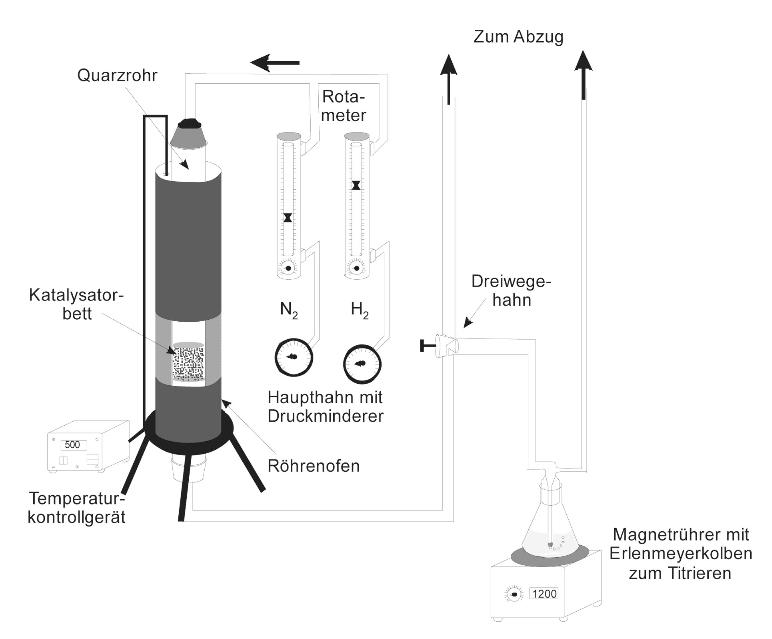
\includegraphics[width=1.0\textwidth]{Versuchsaufbau.png}
  \caption{Schematischer Aufbau der Apparatur zur Ammoniaksynthese. Quelle: Skript S. 28}
  \label{fig:Bild1}
\end{figure}
\subsubsection{Versuchsdurchführung}
Zu erst wurde der Ofen auf 500$^\circ$C vorgeheizt und die Zuleitung für Stickstoff und Wasserstoff geöffnet sowie der Umgebungsdruck abgelesen. Anschließend wurden zu 50 ml einer 5$\cdot10$\textsuperscript{-4} N (2,5$\cdot10$\textsuperscript{-4} M) \ch{H2SO4}-Lösung 5 Tropfen einer Methylrot-Lösung zugegeben(im Erlenmyerkolben). Danach wurde so lange eine NAOH-Lösung dazu gegeben bis ein Umschlag von rot nach zitronengelb stattgefunden hat. Dies dient später beim eigentlichen Versuch zum Vergleich. Bei dem eigentlichen Versuch wurden 4 verschiedene Temperaturen gewählt (hier: 500,570,640 und 700$^\circ$C). Zusätzlich wurde jedes mal ein Erlenmeyerkolben bereitgestellt, gemischt mit 50 ml Schwefelsäure und 5 Tropfen Methylrot plus einen Rührfisch. Diese Mischung wurde beim Gaseinleitungsrohr befestigt durch welches später das entstandene Gas in die Lösung gebracht wurde. Bei jeder Temperatur wurden jeweils 4 Messungen gemacht in welchen jedes mal die Strömungsgeschwindigkeit verändert wurde. Sobald der 3-Wege-Hahn zum Erlenmeyerkolben geöffnet wurde, wurde die Zeit genommen bis ein Farbumschlag sichtbar wurde.
\begin{figure}
	\centering
	\caption{Messwerte}
	\begin{tabular}{c l r r r}
		$T$ in K & Messung & $\dot{V}_{\ch{N2}}$ in $[\frac{\text{Nl}}{\text{h}}]$ & $\dot{V}_{\ch{H2}}$ in $[\frac{\text{Nl}}{\text{h}}]$ & $t$ in [s] \\ \hline \hline
		\multirow{4}{*}{773,15} & 1 & 3,707 & 11,361 & 111 \\
		& 2 & 10,325 & 30,455 & 41 \\
		& 3 & 15,518 & 45,174 & 34 \\
		& 4 & 22,073 & 65,948 & 25 \\ \hline
		\multirow{4}{*}{843,15} & 1 & 3,707 & 11,361 & 156 \\
		& 2 & 10,325 & 30,455 & 68 \\
		& 3 & 15,518 & 45,174 & 47 \\
		& 4 & 22,073 & 65,948 & 33 \\ \hline
		\multirow{4}{*}{913,15} & 1 & 3,707 & 11,361 & 257 \\
		& 2 & 10,325 & 30,455 & 113 \\
		& 3 & 15,518 & 45,174 & 82 \\
		& 4 & 22,073 & 65,948 & 59 \\ \hline
		\multirow{4}{*}{973,15} & 1 & 3,707 & 11,361 & 420 \\
		& 2 & 10,325 & 30,455 & 189 \\
		& 3 & 15,518 & 45,174 & 130 \\
		& 4 & 22,073 & 65,948 & 98 
	\end{tabular}
\end{figure}

\subsubsection{Auswertung}
\textbf{Reaktionsgleichung:}
\ch{1/2 N2 + 3/2 H2 <=> NH3} \\
\textbf{Messwerte:}
Berechnung der Gleichgewichtskonstanten \emph{K\textsubscript{\emph{p}}} mit\\ \\
\begin{equation}
K_p = \frac{ R \cdot T_0 \cdot p_0 \cdot n_{NH\textsubscript{3}} \cdot ( \dot{V}_{N\textsubscript{2}} + \dot{V}_{H\textsubscript{2}})}{\dot{V}^{1/2}_{N\textsubscript{2}} + \dot{V}^{3/2}_{H\textsubscript{2}} \cdot t \cdot p}
\end{equation}
ergibt für die erste Messung:
\begin{equation}
	K_p = \frac{24,337 \;\frac{\text{l} \cdot \text{bar}}{\text{mol}} \cdot 2,5 \cdot 10^{-5} \;\text{mol} \cdot ((\frac{3,707}{3600}) + (\frac{11,361}{3600}))\frac{\text{Nl}}{\text{s}}}{(\frac{3,707}{3600}\frac{\text{Nl}}{\text{s}})^{1/2} + (\frac{11,361}{3600}\frac{\text{Nl}}{\text{s}})^{3/2} \cdot 111 \;\text{s} \cdot 0,968 \;\text{bar}} = 0,00215 = 2,15 \cdot 10^{-3}.
\end{equation}
Es wurde mit R = 0,08319 $\frac{\text{l}\cdot \text{bar}}{\text{mol}\cdot \text{K}}$, T\textsubscript{0} = 293,15 K, p\textsubscript{0} = 1 bar und dem gemessenen Umgebungsdruck von $p = 1,018\; \text{bar} - 0,05 \text{ bar} = 0,968 \text{ bar}$ gerechnet.
\begin{figure}[h]
	\centering
	\caption{Gleichgewichtskonstante $K_p$ und $\ln{K_p}$}
	\begin{tabular}{c|c c|c c|c c|c c}
		$T$ in K & \multicolumn{2}{|c|}{Messung 1} & \multicolumn{2}{c|}{Messung 2} & \multicolumn{2}{c|}{Messung 3} & \multicolumn{2}{c}{Messung 4} \\ \hline \hline
		& $K_p$ & $\ln{K_p}$ & $K_p$ & $\ln{K_p}$ & $K_p$ & $\ln{K_p}$ & $K_p$ & $\ln{K_p}$ \\ \hline
		773,15 & $4,173\cdot 10^{-3}$ & -5,479 & $4,174\cdot 10^{-3}$ &-5,479 & $3,383\cdot 10^{-3}$ & -5,689 & $3,171\cdot 10^{-3}$ & -5,754 \\
		843,15 & $2,969\cdot 10^{-3}$ &-5,819 & $2,517\cdot 10^{-3}$ & -5,985 & $2,447\cdot 10^{-3}$ & -6,013 & $2,403\cdot 10^{-3}$ & -6,031 \\
		913,15 & $1,802\cdot 10^{-3}$ & -6,319 & $1,515\cdot 10^{-3}$ & -6,493 & $1,403\cdot 10^{-3}$ & -6,569 & $1,344\cdot 10^{-3}$ & -6,612 \\
		973,15 & $1,103\cdot 10^{-3}$ & -6,810 & $9,055\cdot 10^{-4}$ & -7,007 & $8,847\cdot 10^{-4}$ & -7,03 & $8,090\cdot 10^{-4}$ & -7,120
	\end{tabular}
\end{figure}

\begin{figure}\label{fig:plot}
	\centering
	\caption{$\ln{K_p}$ über $\frac{1}{T}$}
	% GNUPLOT: LaTeX picture
\setlength{\unitlength}{0.240900pt}
\ifx\plotpoint\undefined\newsavebox{\plotpoint}\fi
\sbox{\plotpoint}{\rule[-0.200pt]{0.400pt}{0.400pt}}%
\begin{picture}(1500,900)(0,0)
\sbox{\plotpoint}{\rule[-0.200pt]{0.400pt}{0.400pt}}%
\put(191.0,131.0){\rule[-0.200pt]{4.818pt}{0.400pt}}
\put(171,131){\makebox(0,0)[r]{$-7$}}
\put(1419.0,131.0){\rule[-0.200pt]{4.818pt}{0.400pt}}
\put(191.0,222.0){\rule[-0.200pt]{4.818pt}{0.400pt}}
\put(171,222){\makebox(0,0)[r]{$-6.8$}}
\put(1419.0,222.0){\rule[-0.200pt]{4.818pt}{0.400pt}}
\put(191.0,313.0){\rule[-0.200pt]{4.818pt}{0.400pt}}
\put(171,313){\makebox(0,0)[r]{$-6.6$}}
\put(1419.0,313.0){\rule[-0.200pt]{4.818pt}{0.400pt}}
\put(191.0,404.0){\rule[-0.200pt]{4.818pt}{0.400pt}}
\put(171,404){\makebox(0,0)[r]{$-6.4$}}
\put(1419.0,404.0){\rule[-0.200pt]{4.818pt}{0.400pt}}
\put(191.0,495.0){\rule[-0.200pt]{4.818pt}{0.400pt}}
\put(171,495){\makebox(0,0)[r]{$-6.2$}}
\put(1419.0,495.0){\rule[-0.200pt]{4.818pt}{0.400pt}}
\put(191.0,586.0){\rule[-0.200pt]{4.818pt}{0.400pt}}
\put(171,586){\makebox(0,0)[r]{$-6$}}
\put(1419.0,586.0){\rule[-0.200pt]{4.818pt}{0.400pt}}
\put(191.0,677.0){\rule[-0.200pt]{4.818pt}{0.400pt}}
\put(171,677){\makebox(0,0)[r]{$-5.8$}}
\put(1419.0,677.0){\rule[-0.200pt]{4.818pt}{0.400pt}}
\put(191.0,768.0){\rule[-0.200pt]{4.818pt}{0.400pt}}
\put(171,768){\makebox(0,0)[r]{$-5.6$}}
\put(1419.0,768.0){\rule[-0.200pt]{4.818pt}{0.400pt}}
\put(191.0,859.0){\rule[-0.200pt]{4.818pt}{0.400pt}}
\put(171,859){\makebox(0,0)[r]{$-5.4$}}
\put(1419.0,859.0){\rule[-0.200pt]{4.818pt}{0.400pt}}
\put(191.0,131.0){\rule[-0.200pt]{0.400pt}{4.818pt}}
\put(191,90){\makebox(0,0){$0.001$}}
\put(191.0,839.0){\rule[-0.200pt]{0.400pt}{4.818pt}}
\put(399.0,131.0){\rule[-0.200pt]{0.400pt}{4.818pt}}
\put(399,90){\makebox(0,0){$0.00105$}}
\put(399.0,839.0){\rule[-0.200pt]{0.400pt}{4.818pt}}
\put(607.0,131.0){\rule[-0.200pt]{0.400pt}{4.818pt}}
\put(607,90){\makebox(0,0){$0.0011$}}
\put(607.0,839.0){\rule[-0.200pt]{0.400pt}{4.818pt}}
\put(815.0,131.0){\rule[-0.200pt]{0.400pt}{4.818pt}}
\put(815,90){\makebox(0,0){$0.00115$}}
\put(815.0,839.0){\rule[-0.200pt]{0.400pt}{4.818pt}}
\put(1023.0,131.0){\rule[-0.200pt]{0.400pt}{4.818pt}}
\put(1023,90){\makebox(0,0){$0.0012$}}
\put(1023.0,839.0){\rule[-0.200pt]{0.400pt}{4.818pt}}
\put(1231.0,131.0){\rule[-0.200pt]{0.400pt}{4.818pt}}
\put(1231,90){\makebox(0,0){$0.00125$}}
\put(1231.0,839.0){\rule[-0.200pt]{0.400pt}{4.818pt}}
\put(1439.0,131.0){\rule[-0.200pt]{0.400pt}{4.818pt}}
\put(1439,90){\makebox(0,0){$0.0013$}}
\put(1439.0,839.0){\rule[-0.200pt]{0.400pt}{4.818pt}}
\put(191.0,131.0){\rule[-0.200pt]{0.400pt}{175.375pt}}
\put(191.0,131.0){\rule[-0.200pt]{300.643pt}{0.400pt}}
\put(1439.0,131.0){\rule[-0.200pt]{0.400pt}{175.375pt}}
\put(191.0,859.0){\rule[-0.200pt]{300.643pt}{0.400pt}}
\put(30,495){\makebox(0,0){ln K}}
\put(815,29){\makebox(0,0){1/T}}
\put(1279,818){\makebox(0,0)[r]{K gemittelt}}
\put(1412,771){\makebox(0,0){$+$}}
\put(965,605){\makebox(0,0){$+$}}
\put(587,362){\makebox(0,0){$+$}}
\put(306,138){\makebox(0,0){$+$}}
\put(1349,818){\makebox(0,0){$+$}}
\put(1279,777){\makebox(0,0)[r]{y = 5219.6804*x -12.2624}}
\put(1299.0,777.0){\rule[-0.200pt]{24.090pt}{0.400pt}}
\put(306,177){\usebox{\plotpoint}}
\multiput(306.00,177.59)(0.943,0.482){9}{\rule{0.833pt}{0.116pt}}
\multiput(306.00,176.17)(9.270,6.000){2}{\rule{0.417pt}{0.400pt}}
\multiput(317.00,183.59)(0.798,0.485){11}{\rule{0.729pt}{0.117pt}}
\multiput(317.00,182.17)(9.488,7.000){2}{\rule{0.364pt}{0.400pt}}
\multiput(328.00,190.59)(0.943,0.482){9}{\rule{0.833pt}{0.116pt}}
\multiput(328.00,189.17)(9.270,6.000){2}{\rule{0.417pt}{0.400pt}}
\multiput(339.00,196.59)(0.798,0.485){11}{\rule{0.729pt}{0.117pt}}
\multiput(339.00,195.17)(9.488,7.000){2}{\rule{0.364pt}{0.400pt}}
\multiput(350.00,203.59)(1.033,0.482){9}{\rule{0.900pt}{0.116pt}}
\multiput(350.00,202.17)(10.132,6.000){2}{\rule{0.450pt}{0.400pt}}
\multiput(362.00,209.59)(0.943,0.482){9}{\rule{0.833pt}{0.116pt}}
\multiput(362.00,208.17)(9.270,6.000){2}{\rule{0.417pt}{0.400pt}}
\multiput(373.00,215.59)(0.798,0.485){11}{\rule{0.729pt}{0.117pt}}
\multiput(373.00,214.17)(9.488,7.000){2}{\rule{0.364pt}{0.400pt}}
\multiput(384.00,222.59)(0.943,0.482){9}{\rule{0.833pt}{0.116pt}}
\multiput(384.00,221.17)(9.270,6.000){2}{\rule{0.417pt}{0.400pt}}
\multiput(395.00,228.59)(0.943,0.482){9}{\rule{0.833pt}{0.116pt}}
\multiput(395.00,227.17)(9.270,6.000){2}{\rule{0.417pt}{0.400pt}}
\multiput(406.00,234.59)(0.798,0.485){11}{\rule{0.729pt}{0.117pt}}
\multiput(406.00,233.17)(9.488,7.000){2}{\rule{0.364pt}{0.400pt}}
\multiput(417.00,241.59)(1.033,0.482){9}{\rule{0.900pt}{0.116pt}}
\multiput(417.00,240.17)(10.132,6.000){2}{\rule{0.450pt}{0.400pt}}
\multiput(429.00,247.59)(0.798,0.485){11}{\rule{0.729pt}{0.117pt}}
\multiput(429.00,246.17)(9.488,7.000){2}{\rule{0.364pt}{0.400pt}}
\multiput(440.00,254.59)(0.943,0.482){9}{\rule{0.833pt}{0.116pt}}
\multiput(440.00,253.17)(9.270,6.000){2}{\rule{0.417pt}{0.400pt}}
\multiput(451.00,260.59)(0.943,0.482){9}{\rule{0.833pt}{0.116pt}}
\multiput(451.00,259.17)(9.270,6.000){2}{\rule{0.417pt}{0.400pt}}
\multiput(462.00,266.59)(0.798,0.485){11}{\rule{0.729pt}{0.117pt}}
\multiput(462.00,265.17)(9.488,7.000){2}{\rule{0.364pt}{0.400pt}}
\multiput(473.00,273.59)(0.943,0.482){9}{\rule{0.833pt}{0.116pt}}
\multiput(473.00,272.17)(9.270,6.000){2}{\rule{0.417pt}{0.400pt}}
\multiput(484.00,279.59)(1.033,0.482){9}{\rule{0.900pt}{0.116pt}}
\multiput(484.00,278.17)(10.132,6.000){2}{\rule{0.450pt}{0.400pt}}
\multiput(496.00,285.59)(0.798,0.485){11}{\rule{0.729pt}{0.117pt}}
\multiput(496.00,284.17)(9.488,7.000){2}{\rule{0.364pt}{0.400pt}}
\multiput(507.00,292.59)(0.943,0.482){9}{\rule{0.833pt}{0.116pt}}
\multiput(507.00,291.17)(9.270,6.000){2}{\rule{0.417pt}{0.400pt}}
\multiput(518.00,298.59)(0.798,0.485){11}{\rule{0.729pt}{0.117pt}}
\multiput(518.00,297.17)(9.488,7.000){2}{\rule{0.364pt}{0.400pt}}
\multiput(529.00,305.59)(0.943,0.482){9}{\rule{0.833pt}{0.116pt}}
\multiput(529.00,304.17)(9.270,6.000){2}{\rule{0.417pt}{0.400pt}}
\multiput(540.00,311.59)(1.033,0.482){9}{\rule{0.900pt}{0.116pt}}
\multiput(540.00,310.17)(10.132,6.000){2}{\rule{0.450pt}{0.400pt}}
\multiput(552.00,317.59)(0.798,0.485){11}{\rule{0.729pt}{0.117pt}}
\multiput(552.00,316.17)(9.488,7.000){2}{\rule{0.364pt}{0.400pt}}
\multiput(563.00,324.59)(0.943,0.482){9}{\rule{0.833pt}{0.116pt}}
\multiput(563.00,323.17)(9.270,6.000){2}{\rule{0.417pt}{0.400pt}}
\multiput(574.00,330.59)(0.943,0.482){9}{\rule{0.833pt}{0.116pt}}
\multiput(574.00,329.17)(9.270,6.000){2}{\rule{0.417pt}{0.400pt}}
\multiput(585.00,336.59)(0.798,0.485){11}{\rule{0.729pt}{0.117pt}}
\multiput(585.00,335.17)(9.488,7.000){2}{\rule{0.364pt}{0.400pt}}
\multiput(596.00,343.59)(0.943,0.482){9}{\rule{0.833pt}{0.116pt}}
\multiput(596.00,342.17)(9.270,6.000){2}{\rule{0.417pt}{0.400pt}}
\multiput(607.00,349.59)(0.874,0.485){11}{\rule{0.786pt}{0.117pt}}
\multiput(607.00,348.17)(10.369,7.000){2}{\rule{0.393pt}{0.400pt}}
\multiput(619.00,356.59)(0.943,0.482){9}{\rule{0.833pt}{0.116pt}}
\multiput(619.00,355.17)(9.270,6.000){2}{\rule{0.417pt}{0.400pt}}
\multiput(630.00,362.59)(0.943,0.482){9}{\rule{0.833pt}{0.116pt}}
\multiput(630.00,361.17)(9.270,6.000){2}{\rule{0.417pt}{0.400pt}}
\multiput(641.00,368.59)(0.798,0.485){11}{\rule{0.729pt}{0.117pt}}
\multiput(641.00,367.17)(9.488,7.000){2}{\rule{0.364pt}{0.400pt}}
\multiput(652.00,375.59)(0.943,0.482){9}{\rule{0.833pt}{0.116pt}}
\multiput(652.00,374.17)(9.270,6.000){2}{\rule{0.417pt}{0.400pt}}
\multiput(663.00,381.59)(0.798,0.485){11}{\rule{0.729pt}{0.117pt}}
\multiput(663.00,380.17)(9.488,7.000){2}{\rule{0.364pt}{0.400pt}}
\multiput(674.00,388.59)(1.033,0.482){9}{\rule{0.900pt}{0.116pt}}
\multiput(674.00,387.17)(10.132,6.000){2}{\rule{0.450pt}{0.400pt}}
\multiput(686.00,394.59)(0.943,0.482){9}{\rule{0.833pt}{0.116pt}}
\multiput(686.00,393.17)(9.270,6.000){2}{\rule{0.417pt}{0.400pt}}
\multiput(697.00,400.59)(0.798,0.485){11}{\rule{0.729pt}{0.117pt}}
\multiput(697.00,399.17)(9.488,7.000){2}{\rule{0.364pt}{0.400pt}}
\multiput(708.00,407.59)(0.943,0.482){9}{\rule{0.833pt}{0.116pt}}
\multiput(708.00,406.17)(9.270,6.000){2}{\rule{0.417pt}{0.400pt}}
\multiput(719.00,413.59)(0.943,0.482){9}{\rule{0.833pt}{0.116pt}}
\multiput(719.00,412.17)(9.270,6.000){2}{\rule{0.417pt}{0.400pt}}
\multiput(730.00,419.59)(0.798,0.485){11}{\rule{0.729pt}{0.117pt}}
\multiput(730.00,418.17)(9.488,7.000){2}{\rule{0.364pt}{0.400pt}}
\multiput(741.00,426.59)(1.033,0.482){9}{\rule{0.900pt}{0.116pt}}
\multiput(741.00,425.17)(10.132,6.000){2}{\rule{0.450pt}{0.400pt}}
\multiput(753.00,432.59)(0.798,0.485){11}{\rule{0.729pt}{0.117pt}}
\multiput(753.00,431.17)(9.488,7.000){2}{\rule{0.364pt}{0.400pt}}
\multiput(764.00,439.59)(0.943,0.482){9}{\rule{0.833pt}{0.116pt}}
\multiput(764.00,438.17)(9.270,6.000){2}{\rule{0.417pt}{0.400pt}}
\multiput(775.00,445.59)(0.943,0.482){9}{\rule{0.833pt}{0.116pt}}
\multiput(775.00,444.17)(9.270,6.000){2}{\rule{0.417pt}{0.400pt}}
\multiput(786.00,451.59)(0.798,0.485){11}{\rule{0.729pt}{0.117pt}}
\multiput(786.00,450.17)(9.488,7.000){2}{\rule{0.364pt}{0.400pt}}
\multiput(797.00,458.59)(0.943,0.482){9}{\rule{0.833pt}{0.116pt}}
\multiput(797.00,457.17)(9.270,6.000){2}{\rule{0.417pt}{0.400pt}}
\multiput(808.00,464.59)(1.033,0.482){9}{\rule{0.900pt}{0.116pt}}
\multiput(808.00,463.17)(10.132,6.000){2}{\rule{0.450pt}{0.400pt}}
\multiput(820.00,470.59)(0.798,0.485){11}{\rule{0.729pt}{0.117pt}}
\multiput(820.00,469.17)(9.488,7.000){2}{\rule{0.364pt}{0.400pt}}
\multiput(831.00,477.59)(0.943,0.482){9}{\rule{0.833pt}{0.116pt}}
\multiput(831.00,476.17)(9.270,6.000){2}{\rule{0.417pt}{0.400pt}}
\multiput(842.00,483.59)(0.798,0.485){11}{\rule{0.729pt}{0.117pt}}
\multiput(842.00,482.17)(9.488,7.000){2}{\rule{0.364pt}{0.400pt}}
\multiput(853.00,490.59)(0.943,0.482){9}{\rule{0.833pt}{0.116pt}}
\multiput(853.00,489.17)(9.270,6.000){2}{\rule{0.417pt}{0.400pt}}
\multiput(864.00,496.59)(0.943,0.482){9}{\rule{0.833pt}{0.116pt}}
\multiput(864.00,495.17)(9.270,6.000){2}{\rule{0.417pt}{0.400pt}}
\multiput(875.00,502.59)(0.874,0.485){11}{\rule{0.786pt}{0.117pt}}
\multiput(875.00,501.17)(10.369,7.000){2}{\rule{0.393pt}{0.400pt}}
\multiput(887.00,509.59)(0.943,0.482){9}{\rule{0.833pt}{0.116pt}}
\multiput(887.00,508.17)(9.270,6.000){2}{\rule{0.417pt}{0.400pt}}
\multiput(898.00,515.59)(0.943,0.482){9}{\rule{0.833pt}{0.116pt}}
\multiput(898.00,514.17)(9.270,6.000){2}{\rule{0.417pt}{0.400pt}}
\multiput(909.00,521.59)(0.798,0.485){11}{\rule{0.729pt}{0.117pt}}
\multiput(909.00,520.17)(9.488,7.000){2}{\rule{0.364pt}{0.400pt}}
\multiput(920.00,528.59)(0.943,0.482){9}{\rule{0.833pt}{0.116pt}}
\multiput(920.00,527.17)(9.270,6.000){2}{\rule{0.417pt}{0.400pt}}
\multiput(931.00,534.59)(0.798,0.485){11}{\rule{0.729pt}{0.117pt}}
\multiput(931.00,533.17)(9.488,7.000){2}{\rule{0.364pt}{0.400pt}}
\multiput(942.00,541.59)(1.033,0.482){9}{\rule{0.900pt}{0.116pt}}
\multiput(942.00,540.17)(10.132,6.000){2}{\rule{0.450pt}{0.400pt}}
\multiput(954.00,547.59)(0.943,0.482){9}{\rule{0.833pt}{0.116pt}}
\multiput(954.00,546.17)(9.270,6.000){2}{\rule{0.417pt}{0.400pt}}
\multiput(965.00,553.59)(0.798,0.485){11}{\rule{0.729pt}{0.117pt}}
\multiput(965.00,552.17)(9.488,7.000){2}{\rule{0.364pt}{0.400pt}}
\multiput(976.00,560.59)(0.943,0.482){9}{\rule{0.833pt}{0.116pt}}
\multiput(976.00,559.17)(9.270,6.000){2}{\rule{0.417pt}{0.400pt}}
\multiput(987.00,566.59)(0.943,0.482){9}{\rule{0.833pt}{0.116pt}}
\multiput(987.00,565.17)(9.270,6.000){2}{\rule{0.417pt}{0.400pt}}
\multiput(998.00,572.59)(0.798,0.485){11}{\rule{0.729pt}{0.117pt}}
\multiput(998.00,571.17)(9.488,7.000){2}{\rule{0.364pt}{0.400pt}}
\multiput(1009.00,579.59)(1.033,0.482){9}{\rule{0.900pt}{0.116pt}}
\multiput(1009.00,578.17)(10.132,6.000){2}{\rule{0.450pt}{0.400pt}}
\multiput(1021.00,585.59)(0.798,0.485){11}{\rule{0.729pt}{0.117pt}}
\multiput(1021.00,584.17)(9.488,7.000){2}{\rule{0.364pt}{0.400pt}}
\multiput(1032.00,592.59)(0.943,0.482){9}{\rule{0.833pt}{0.116pt}}
\multiput(1032.00,591.17)(9.270,6.000){2}{\rule{0.417pt}{0.400pt}}
\multiput(1043.00,598.59)(0.943,0.482){9}{\rule{0.833pt}{0.116pt}}
\multiput(1043.00,597.17)(9.270,6.000){2}{\rule{0.417pt}{0.400pt}}
\multiput(1054.00,604.59)(0.798,0.485){11}{\rule{0.729pt}{0.117pt}}
\multiput(1054.00,603.17)(9.488,7.000){2}{\rule{0.364pt}{0.400pt}}
\multiput(1065.00,611.59)(0.943,0.482){9}{\rule{0.833pt}{0.116pt}}
\multiput(1065.00,610.17)(9.270,6.000){2}{\rule{0.417pt}{0.400pt}}
\multiput(1076.00,617.59)(1.033,0.482){9}{\rule{0.900pt}{0.116pt}}
\multiput(1076.00,616.17)(10.132,6.000){2}{\rule{0.450pt}{0.400pt}}
\multiput(1088.00,623.59)(0.798,0.485){11}{\rule{0.729pt}{0.117pt}}
\multiput(1088.00,622.17)(9.488,7.000){2}{\rule{0.364pt}{0.400pt}}
\multiput(1099.00,630.59)(0.943,0.482){9}{\rule{0.833pt}{0.116pt}}
\multiput(1099.00,629.17)(9.270,6.000){2}{\rule{0.417pt}{0.400pt}}
\multiput(1110.00,636.59)(0.798,0.485){11}{\rule{0.729pt}{0.117pt}}
\multiput(1110.00,635.17)(9.488,7.000){2}{\rule{0.364pt}{0.400pt}}
\multiput(1121.00,643.59)(0.943,0.482){9}{\rule{0.833pt}{0.116pt}}
\multiput(1121.00,642.17)(9.270,6.000){2}{\rule{0.417pt}{0.400pt}}
\multiput(1132.00,649.59)(1.033,0.482){9}{\rule{0.900pt}{0.116pt}}
\multiput(1132.00,648.17)(10.132,6.000){2}{\rule{0.450pt}{0.400pt}}
\multiput(1144.00,655.59)(0.798,0.485){11}{\rule{0.729pt}{0.117pt}}
\multiput(1144.00,654.17)(9.488,7.000){2}{\rule{0.364pt}{0.400pt}}
\multiput(1155.00,662.59)(0.943,0.482){9}{\rule{0.833pt}{0.116pt}}
\multiput(1155.00,661.17)(9.270,6.000){2}{\rule{0.417pt}{0.400pt}}
\multiput(1166.00,668.59)(0.943,0.482){9}{\rule{0.833pt}{0.116pt}}
\multiput(1166.00,667.17)(9.270,6.000){2}{\rule{0.417pt}{0.400pt}}
\multiput(1177.00,674.59)(0.798,0.485){11}{\rule{0.729pt}{0.117pt}}
\multiput(1177.00,673.17)(9.488,7.000){2}{\rule{0.364pt}{0.400pt}}
\multiput(1188.00,681.59)(0.943,0.482){9}{\rule{0.833pt}{0.116pt}}
\multiput(1188.00,680.17)(9.270,6.000){2}{\rule{0.417pt}{0.400pt}}
\multiput(1199.00,687.59)(0.874,0.485){11}{\rule{0.786pt}{0.117pt}}
\multiput(1199.00,686.17)(10.369,7.000){2}{\rule{0.393pt}{0.400pt}}
\multiput(1211.00,694.59)(0.943,0.482){9}{\rule{0.833pt}{0.116pt}}
\multiput(1211.00,693.17)(9.270,6.000){2}{\rule{0.417pt}{0.400pt}}
\multiput(1222.00,700.59)(0.943,0.482){9}{\rule{0.833pt}{0.116pt}}
\multiput(1222.00,699.17)(9.270,6.000){2}{\rule{0.417pt}{0.400pt}}
\multiput(1233.00,706.59)(0.798,0.485){11}{\rule{0.729pt}{0.117pt}}
\multiput(1233.00,705.17)(9.488,7.000){2}{\rule{0.364pt}{0.400pt}}
\multiput(1244.00,713.59)(0.943,0.482){9}{\rule{0.833pt}{0.116pt}}
\multiput(1244.00,712.17)(9.270,6.000){2}{\rule{0.417pt}{0.400pt}}
\multiput(1255.00,719.59)(0.943,0.482){9}{\rule{0.833pt}{0.116pt}}
\multiput(1255.00,718.17)(9.270,6.000){2}{\rule{0.417pt}{0.400pt}}
\multiput(1266.00,725.59)(0.874,0.485){11}{\rule{0.786pt}{0.117pt}}
\multiput(1266.00,724.17)(10.369,7.000){2}{\rule{0.393pt}{0.400pt}}
\multiput(1278.00,732.59)(0.943,0.482){9}{\rule{0.833pt}{0.116pt}}
\multiput(1278.00,731.17)(9.270,6.000){2}{\rule{0.417pt}{0.400pt}}
\multiput(1289.00,738.59)(0.798,0.485){11}{\rule{0.729pt}{0.117pt}}
\multiput(1289.00,737.17)(9.488,7.000){2}{\rule{0.364pt}{0.400pt}}
\multiput(1300.00,745.59)(0.943,0.482){9}{\rule{0.833pt}{0.116pt}}
\multiput(1300.00,744.17)(9.270,6.000){2}{\rule{0.417pt}{0.400pt}}
\multiput(1311.00,751.59)(0.943,0.482){9}{\rule{0.833pt}{0.116pt}}
\multiput(1311.00,750.17)(9.270,6.000){2}{\rule{0.417pt}{0.400pt}}
\multiput(1322.00,757.59)(0.798,0.485){11}{\rule{0.729pt}{0.117pt}}
\multiput(1322.00,756.17)(9.488,7.000){2}{\rule{0.364pt}{0.400pt}}
\multiput(1333.00,764.59)(1.033,0.482){9}{\rule{0.900pt}{0.116pt}}
\multiput(1333.00,763.17)(10.132,6.000){2}{\rule{0.450pt}{0.400pt}}
\multiput(1345.00,770.59)(0.798,0.485){11}{\rule{0.729pt}{0.117pt}}
\multiput(1345.00,769.17)(9.488,7.000){2}{\rule{0.364pt}{0.400pt}}
\multiput(1356.00,777.59)(0.943,0.482){9}{\rule{0.833pt}{0.116pt}}
\multiput(1356.00,776.17)(9.270,6.000){2}{\rule{0.417pt}{0.400pt}}
\multiput(1367.00,783.59)(0.943,0.482){9}{\rule{0.833pt}{0.116pt}}
\multiput(1367.00,782.17)(9.270,6.000){2}{\rule{0.417pt}{0.400pt}}
\multiput(1378.00,789.59)(0.798,0.485){11}{\rule{0.729pt}{0.117pt}}
\multiput(1378.00,788.17)(9.488,7.000){2}{\rule{0.364pt}{0.400pt}}
\multiput(1389.00,796.59)(0.943,0.482){9}{\rule{0.833pt}{0.116pt}}
\multiput(1389.00,795.17)(9.270,6.000){2}{\rule{0.417pt}{0.400pt}}
\multiput(1400.00,802.59)(1.033,0.482){9}{\rule{0.900pt}{0.116pt}}
\multiput(1400.00,801.17)(10.132,6.000){2}{\rule{0.450pt}{0.400pt}}
\put(191.0,131.0){\rule[-0.200pt]{0.400pt}{175.375pt}}
\put(191.0,131.0){\rule[-0.200pt]{300.643pt}{0.400pt}}
\put(1439.0,131.0){\rule[-0.200pt]{0.400pt}{175.375pt}}
\put(191.0,859.0){\rule[-0.200pt]{300.643pt}{0.400pt}}
\end{picture}

\end{figure}
Mittelt man nun jeweils die vier errechneten $K_p$, bzw $\ln{K_p}$ für eine Temperatur und plottet diese gemittelten $\ln{K_p}$ über die jeweils entsprechende reziproke Temperatur erhält man Abbildung~\ref{fig:plot} mit einer gefitteten y Kurve, die der Gleichung~\ref{eq:lnK2} mit Steigung $-\frac{\Delta_r H^0}{R} = 5219,6804$ entspricht. Daraus errechnet sich eine Reaktionsenthalpie $\Delta_r H^0 = -R\cdot 5219,6804= -43398,8229 \frac{\text{J}}{\text{mol}}$. Die Reaktionenthalpie zur Reaktionsgleichung \ch{N2 + 3 H2 <=> 2 NH3} beträgt nach Literaturangaben\footnote{\url{https://de.wikipedia.org/wiki/Haber-Bosch-Verfahren#Synthesebedingungen}} $\Delta H_{2\ch{NH3}} = -92,28$ kJ. Daraus folgt eine Reaktionsenthalpie $\Delta H_{\ch{NH3}} =\frac{1}{2} \Delta H_{2\ch{NH3}} = -46,14$ kJ für die Reaktion \ch{1/2 N2 + 3/2 H2 <=> NH3}. Die Abweichung von diesem Wert und dem gemessenen liegt bei etwa $5,94\%$.
\section{Literatur}
\begin{enumerate}[label=(\arabic*)]
	\item \emph{Praktische Einführung in die Chemie
für Studierende der Fachrichtungen
Technische Biologie und Physik}. Praktikumsskript, Universität Stuttgart,
SoSe 2017.  
	\item Prof. Dr. D. Gudat. \emph{„Einführung in die Chemie für Naturwissenschaftler“}. Vorlesungsskript
	\item \emph{Das Basiswissen der Chemie}. Charles E. Mortimer, Ulrich Müller. 12. Auflage
\end{enumerate}
\end{document}		
